% Anchor blueprint-pair diagram: two tilted planes representing the
% informal (red, top) and formal (blue, bottom) dependency graphs, linked
% by blueprint \lean{} annotations (green dashed).
%
% Story:
%   - Anchor = an informal blueprint statement A with a \lean{}-resolved
%     formal partner A on the bottom plane.
%   - k=1 informal neighbors of A: TWO are UNFORMALIZED (outlined red,
%     no formal partner). ONE is FORMALIZED (filled red, paired with a
%     blue node via a dashed green \lean{} link).
%   - One k=2 informal neighbor (reached via the formalized k=1 node)
%     is also formalized — but further from the anchor.
%
% This is the canonical figure for the §11 dual-plane theme in
% figure_style.md.
%
% Build:  pdflatex anchor_neighborhood.tex
% Output: ../out/anchor_neighborhood.pdf

\documentclass[tikz,border=8pt]{standalone}
\usepackage{tikz}
\usetikzlibrary{positioning,arrows.meta,calc,backgrounds}

% --- Palette (figure_style.md §2) ----------------------------------------
\definecolor{BluePrimary}{HTML}{2E5C8A}
\definecolor{AccentRed}{HTML}{C8553D}
\definecolor{AccentGreen}{HTML}{5B8C5A}
\definecolor{GrayText}{HTML}{2A2A2A}
\definecolor{GrayRule}{HTML}{999999}

% --- Styles (§11 dual-plane theme) ---------------------------------------
\tikzset{
  every node/.style       = {font=\sffamily\small, text=GrayText},
  inode/.style            = {circle, draw=AccentRed!85, fill=AccentRed!80,
                             line width=0.6pt, minimum size=5mm, inner sep=0pt,
                             text=white, font=\sffamily\bfseries\scriptsize},
  inode_unform/.style     = {inode, fill=AccentRed!8, text=AccentRed,
                             line width=1.4pt},
  fnode/.style            = {circle, draw=BluePrimary, fill=BluePrimary!85,
                             line width=0.6pt, minimum size=5mm, inner sep=0pt,
                             text=white, font=\sffamily\bfseries\scriptsize},
  ianchor/.style          = {inode, minimum size=7.5mm, line width=1.0pt,
                             font=\sffamily\bfseries\small},
  fanchor/.style          = {fnode, minimum size=7.5mm, line width=1.0pt,
                             font=\sffamily\bfseries\small},
  iedge/.style            = {-, line width=0.6pt, draw=AccentRed!60},
  fedge/.style            = {-, line width=0.6pt, draw=BluePrimary!70},
  blueprint/.style        = {densely dashed, line width=0.55pt,
                             draw=AccentGreen!85},
  blueprint_anchor/.style = {blueprint, line width=1.2pt, draw=AccentGreen},
  plane_top/.style        = {fill=AccentRed!4,    draw=AccentRed!28,
                             line width=0.4pt},
  plane_bot/.style        = {fill=BluePrimary!4,  draw=BluePrimary!28,
                             line width=0.4pt},
}

% --- Plane geometry (shear gives the slight 3D tilt) ---------------------
\def\PlaneW{7.4}
\def\Dx{1.5}
\def\Dy{0.95}
\def\TopY{5.2}
\def\BotY{0}

\begin{document}
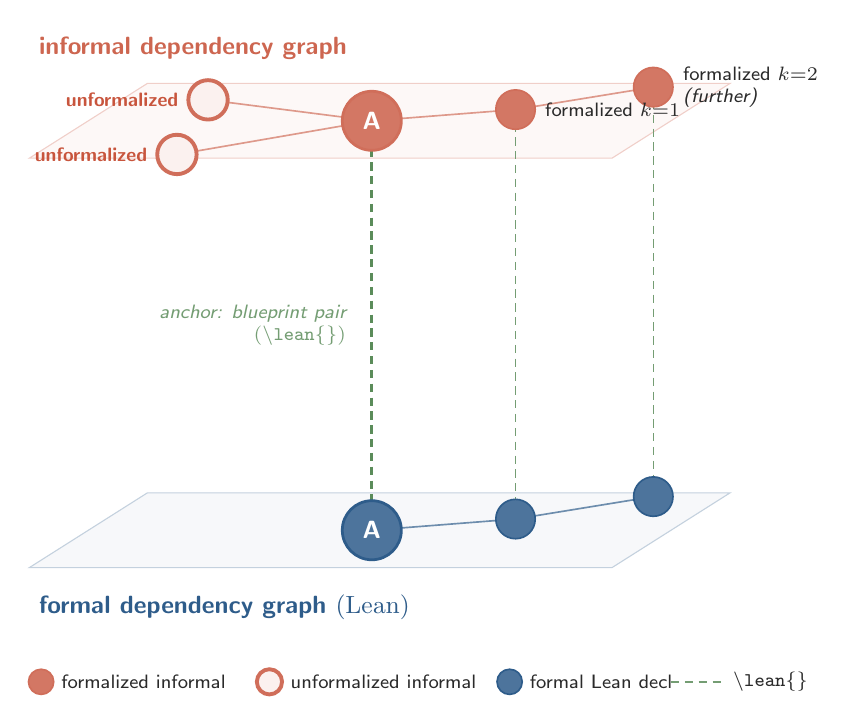
\begin{tikzpicture}[x=1cm, y=1cm]

% =========================================================================
% Plane parallelograms
% =========================================================================
\draw[plane_top]
   (0, \TopY) -- (\PlaneW, \TopY)
   -- ($(\PlaneW, \TopY) + (\Dx, \Dy)$) -- ($(0, \TopY) + (\Dx, \Dy)$) -- cycle;
\draw[plane_bot]
   (0, \BotY) -- (\PlaneW, \BotY)
   -- ($(\PlaneW, \BotY) + (\Dx, \Dy)$) -- ($(0, \BotY) + (\Dx, \Dy)$) -- cycle;

% --- Plane labels (placed OUTSIDE the parallelograms) --------------------
\node[anchor=west, text=AccentRed!90,
      font=\sffamily\bfseries\small\itshape]
  at (0, \TopY + \Dy + 0.45)
  {informal dependency graph};
\node[anchor=west, text=BluePrimary,
      font=\sffamily\bfseries\small\itshape]
  at (0, \BotY - 0.50)
  {formal dependency graph \textnormal{(Lean)}};

% =========================================================================
% Node coordinates  (plane-local u, v -> world: x = u + v*Dx, y = py + v*Dy)
% =========================================================================
% Informal (top)
\coordinate (Ai) at (3.6 + 0.50*\Dx, \TopY + 0.50*\Dy);   % anchor
\coordinate (N1) at (1.1 + 0.78*\Dx, \TopY + 0.78*\Dy);   % unformalized
\coordinate (N2) at (1.8 + 0.05*\Dx, \TopY + 0.05*\Dy);   % unformalized
\coordinate (N3) at (5.2 + 0.65*\Dx, \TopY + 0.65*\Dy);   % formalized k=1
\coordinate (N4) at (6.5 + 0.95*\Dx, \TopY + 0.95*\Dy);   % formalized k=2

% Formal (bottom): only the nodes that have informal partners
\coordinate (Af)  at (3.6 + 0.50*\Dx, \BotY + 0.50*\Dy);
\coordinate (N3f) at (5.2 + 0.65*\Dx, \BotY + 0.65*\Dy);
\coordinate (N4f) at (6.5 + 0.95*\Dx, \BotY + 0.95*\Dy);

% =========================================================================
% Edges (drawn before nodes so fills sit on top)
% =========================================================================
\draw[iedge] (Ai) -- (N1);
\draw[iedge] (Ai) -- (N2);
\draw[iedge] (Ai) -- (N3);
\draw[iedge] (N3) -- (N4);

\draw[fedge] (Af) -- (N3f);
\draw[fedge] (N3f) -- (N4f);

\draw[blueprint_anchor] (Ai) -- (Af);
\draw[blueprint]        (N3) -- (N3f);
\draw[blueprint]        (N4) -- (N4f);

% =========================================================================
% Nodes
% =========================================================================
\node[ianchor]      at (Ai)  {A};
\node[inode_unform] at (N1)  {};
\node[inode_unform] at (N2)  {};
\node[inode]        at (N3)  {};
\node[inode]        at (N4)  {};

\node[fanchor]      at (Af)  {A};
\node[fnode]        at (N3f) {};
\node[fnode]        at (N4f) {};

% =========================================================================
% Annotations
% =========================================================================
% Anchor pair label (between the planes, left of the green vertical link)
\node[anchor=east, font=\sffamily\scriptsize\itshape, text=AccentGreen!85,
      align=right, inner sep=2pt]
  at ($(Ai)!0.5!(Af) + (-0.25, 0)$)
  {anchor: blueprint pair\\\textnormal{(\texttt{\textbackslash lean\{\}})}};

% Unformalized labels (red, bold, anchored to the LEFT of each node)
\node[anchor=east, font=\sffamily\scriptsize\bfseries, text=AccentRed,
      inner sep=2pt]
  at ($(N1) + (-0.30, 0)$) {unformalized};
\node[anchor=east, font=\sffamily\scriptsize\bfseries, text=AccentRed,
      inner sep=2pt]
  at ($(N2) + (-0.30, 0)$) {unformalized};

% N3 (formalized k=1) and N4 (formalized k=2) labels — to the right side
\node[anchor=west, font=\sffamily\scriptsize, text=GrayText,
      inner sep=2pt]
  at ($(N3) + (0.30, 0)$) {formalized $k{=}1$};
\node[anchor=west, font=\sffamily\scriptsize, text=GrayText,
      align=left, inner sep=2pt]
  at ($(N4) + (0.30, 0)$) {formalized $k{=}2$\\\textit{(further)}};

% =========================================================================
% Legend  (compact, single row, below the bottom plane label)
% =========================================================================
\begin{scope}[shift={(0, -1.45)}]
  \node[inode, minimum size=3.2mm] (lg1) at (0.15, 0) {};
  \node[anchor=west, font=\sffamily\scriptsize, inner sep=1pt]
    at (lg1.east) {\,formalized informal};

  \node[inode_unform, minimum size=3.2mm] (lg2) at (3.05, 0) {};
  \node[anchor=west, font=\sffamily\scriptsize, inner sep=1pt]
    at (lg2.east) {\,unformalized informal};

  \node[fnode, minimum size=3.2mm] (lg3) at (6.10, 0) {};
  \node[anchor=west, font=\sffamily\scriptsize, inner sep=1pt]
    at (lg3.east) {\,formal Lean decl};

  \draw[blueprint, line width=0.9pt] (8.15, 0) -- (8.85, 0);
  \node[anchor=west, font=\sffamily\scriptsize, inner sep=1pt]
    at (8.85, 0) {\,\texttt{\textbackslash lean\{\}}};
\end{scope}

\end{tikzpicture}
\end{document}
